\documentclass{article}\usepackage[]{graphicx}\usepackage[]{color}
%% maxwidth is the original width if it is less than linewidth
%% otherwise use linewidth (to make sure the graphics do not exceed the margin)
\makeatletter
\def\maxwidth{ %
  \ifdim\Gin@nat@width>\linewidth
    \linewidth
  \else
    \Gin@nat@width
  \fi
}
\makeatother

\definecolor{fgcolor}{rgb}{0.345, 0.345, 0.345}
\newcommand{\hlnum}[1]{\textcolor[rgb]{0.686,0.059,0.569}{#1}}%
\newcommand{\hlstr}[1]{\textcolor[rgb]{0.192,0.494,0.8}{#1}}%
\newcommand{\hlcom}[1]{\textcolor[rgb]{0.678,0.584,0.686}{\textit{#1}}}%
\newcommand{\hlopt}[1]{\textcolor[rgb]{0,0,0}{#1}}%
\newcommand{\hlstd}[1]{\textcolor[rgb]{0.345,0.345,0.345}{#1}}%
\newcommand{\hlkwa}[1]{\textcolor[rgb]{0.161,0.373,0.58}{\textbf{#1}}}%
\newcommand{\hlkwb}[1]{\textcolor[rgb]{0.69,0.353,0.396}{#1}}%
\newcommand{\hlkwc}[1]{\textcolor[rgb]{0.333,0.667,0.333}{#1}}%
\newcommand{\hlkwd}[1]{\textcolor[rgb]{0.737,0.353,0.396}{\textbf{#1}}}%
\let\hlipl\hlkwb

\usepackage{framed}
\makeatletter
\newenvironment{kframe}{%
 \def\at@end@of@kframe{}%
 \ifinner\ifhmode%
  \def\at@end@of@kframe{\end{minipage}}%
  \begin{minipage}{\columnwidth}%
 \fi\fi%
 \def\FrameCommand##1{\hskip\@totalleftmargin \hskip-\fboxsep
 \colorbox{shadecolor}{##1}\hskip-\fboxsep
     % There is no \\@totalrightmargin, so:
     \hskip-\linewidth \hskip-\@totalleftmargin \hskip\columnwidth}%
 \MakeFramed {\advance\hsize-\width
   \@totalleftmargin\z@ \linewidth\hsize
   \@setminipage}}%
 {\par\unskip\endMakeFramed%
 \at@end@of@kframe}
\makeatother

\definecolor{shadecolor}{rgb}{.97, .97, .97}
\definecolor{messagecolor}{rgb}{0, 0, 0}
\definecolor{warningcolor}{rgb}{1, 0, 1}
\definecolor{errorcolor}{rgb}{1, 0, 0}
\newenvironment{knitrout}{}{} % an empty environment to be redefined in TeX

\usepackage{alltt}
\usepackage{enumitem}
\usepackage{ amssymb }
\usepackage{ textcomp }
\usepackage{longtable}
\usepackage{amsmath,tabu}


\topmargin=-0.45in
\evensidemargin=0in
\oddsidemargin=0in
\textwidth=6.5in
\textheight=9.0in
\headsep=0.25in

\title{Cross Correlation Analyses}
\author{Caleb Lareau}
\date{\today}
\IfFileExists{upquote.sty}{\usepackage{upquote}}{}
\begin{document}
\maketitle

\section*{Introduction}
The basic problem that is examined is the modeling of the relationship between two time-dependent variables wherein a potential ``lag" may be observed. For example, one may expect the price of crude oil to be correlated with the currency conversation rate between the Saudi riyal and US dollar. Howevever, the best correlation between these variables is likely observed after some delay. In this example, the price of crude oil plummetting one day could may be correlated with a depleted riyal/USD conversion rate after another 2-3 days. For my final project, I propose to examine the statistical estimation procedure and utilities available in \texttt{R} to examine time-varying variables in the context of lag. I will explore the utility of these stastical forms in the context of single-cell biological data. 

\section*{Statistics}
For continuous functions $f$ and $g$, the cross-correlation is defined as:
$$(f\star g)(\tau )\ {\stackrel {\mathrm {def} }{=}}\int _{-\infty }^{\infty }f(t)\ g(t+\tau )\,dt$$
where the optimal lag is defined as:
$$ \tau _{\mathrm {delay} }={\underset {t}{\operatorname {arg\,max} }}((f\star g)(t))$$

\noindent In the context of real data, $f$ and $g$ will not be continuous, but discrete functions, and the cross-correlation can similarly be computed.

\section*{Intended Application}
In gene regulation, regions of DNA called "enhancers" 

 \textbf{Figure \ref{fig:one}}
 
 \begin{figure}[ht]
    \centering
    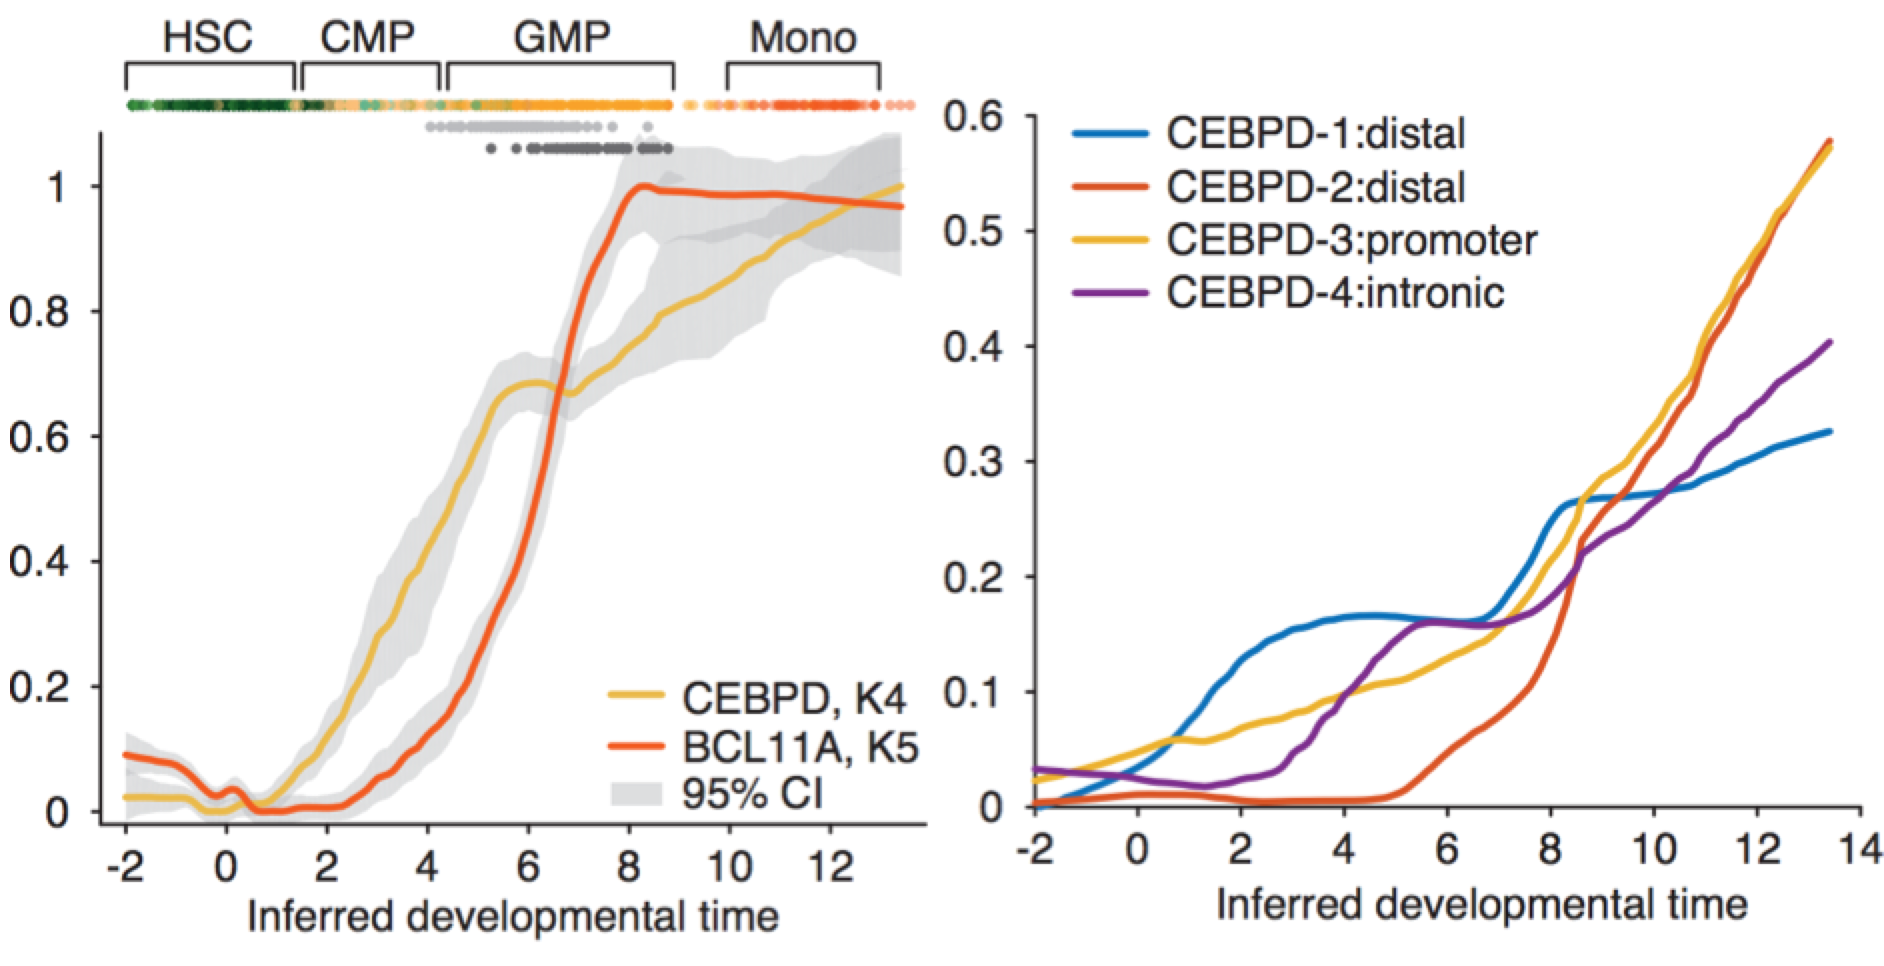
\includegraphics[width=\textwidth]{zero.png}
    \caption{\textbf{A graphical overview of single-cell data.} In the plot to the left, a measure of total intensity (for simplicity, think gene expression) of two genes, including CEBPD. This plot shows that this gene is lowly expressed in stem cells (to the left), but highly expressed in monocytes (to the right). Each point represents a single cell where data is observed. In the plot on the right, four different enhancer activity scores are plotted. }
    \label{fig:zero}
\end{figure}
 
\begin{figure}[ht]
    \centering
    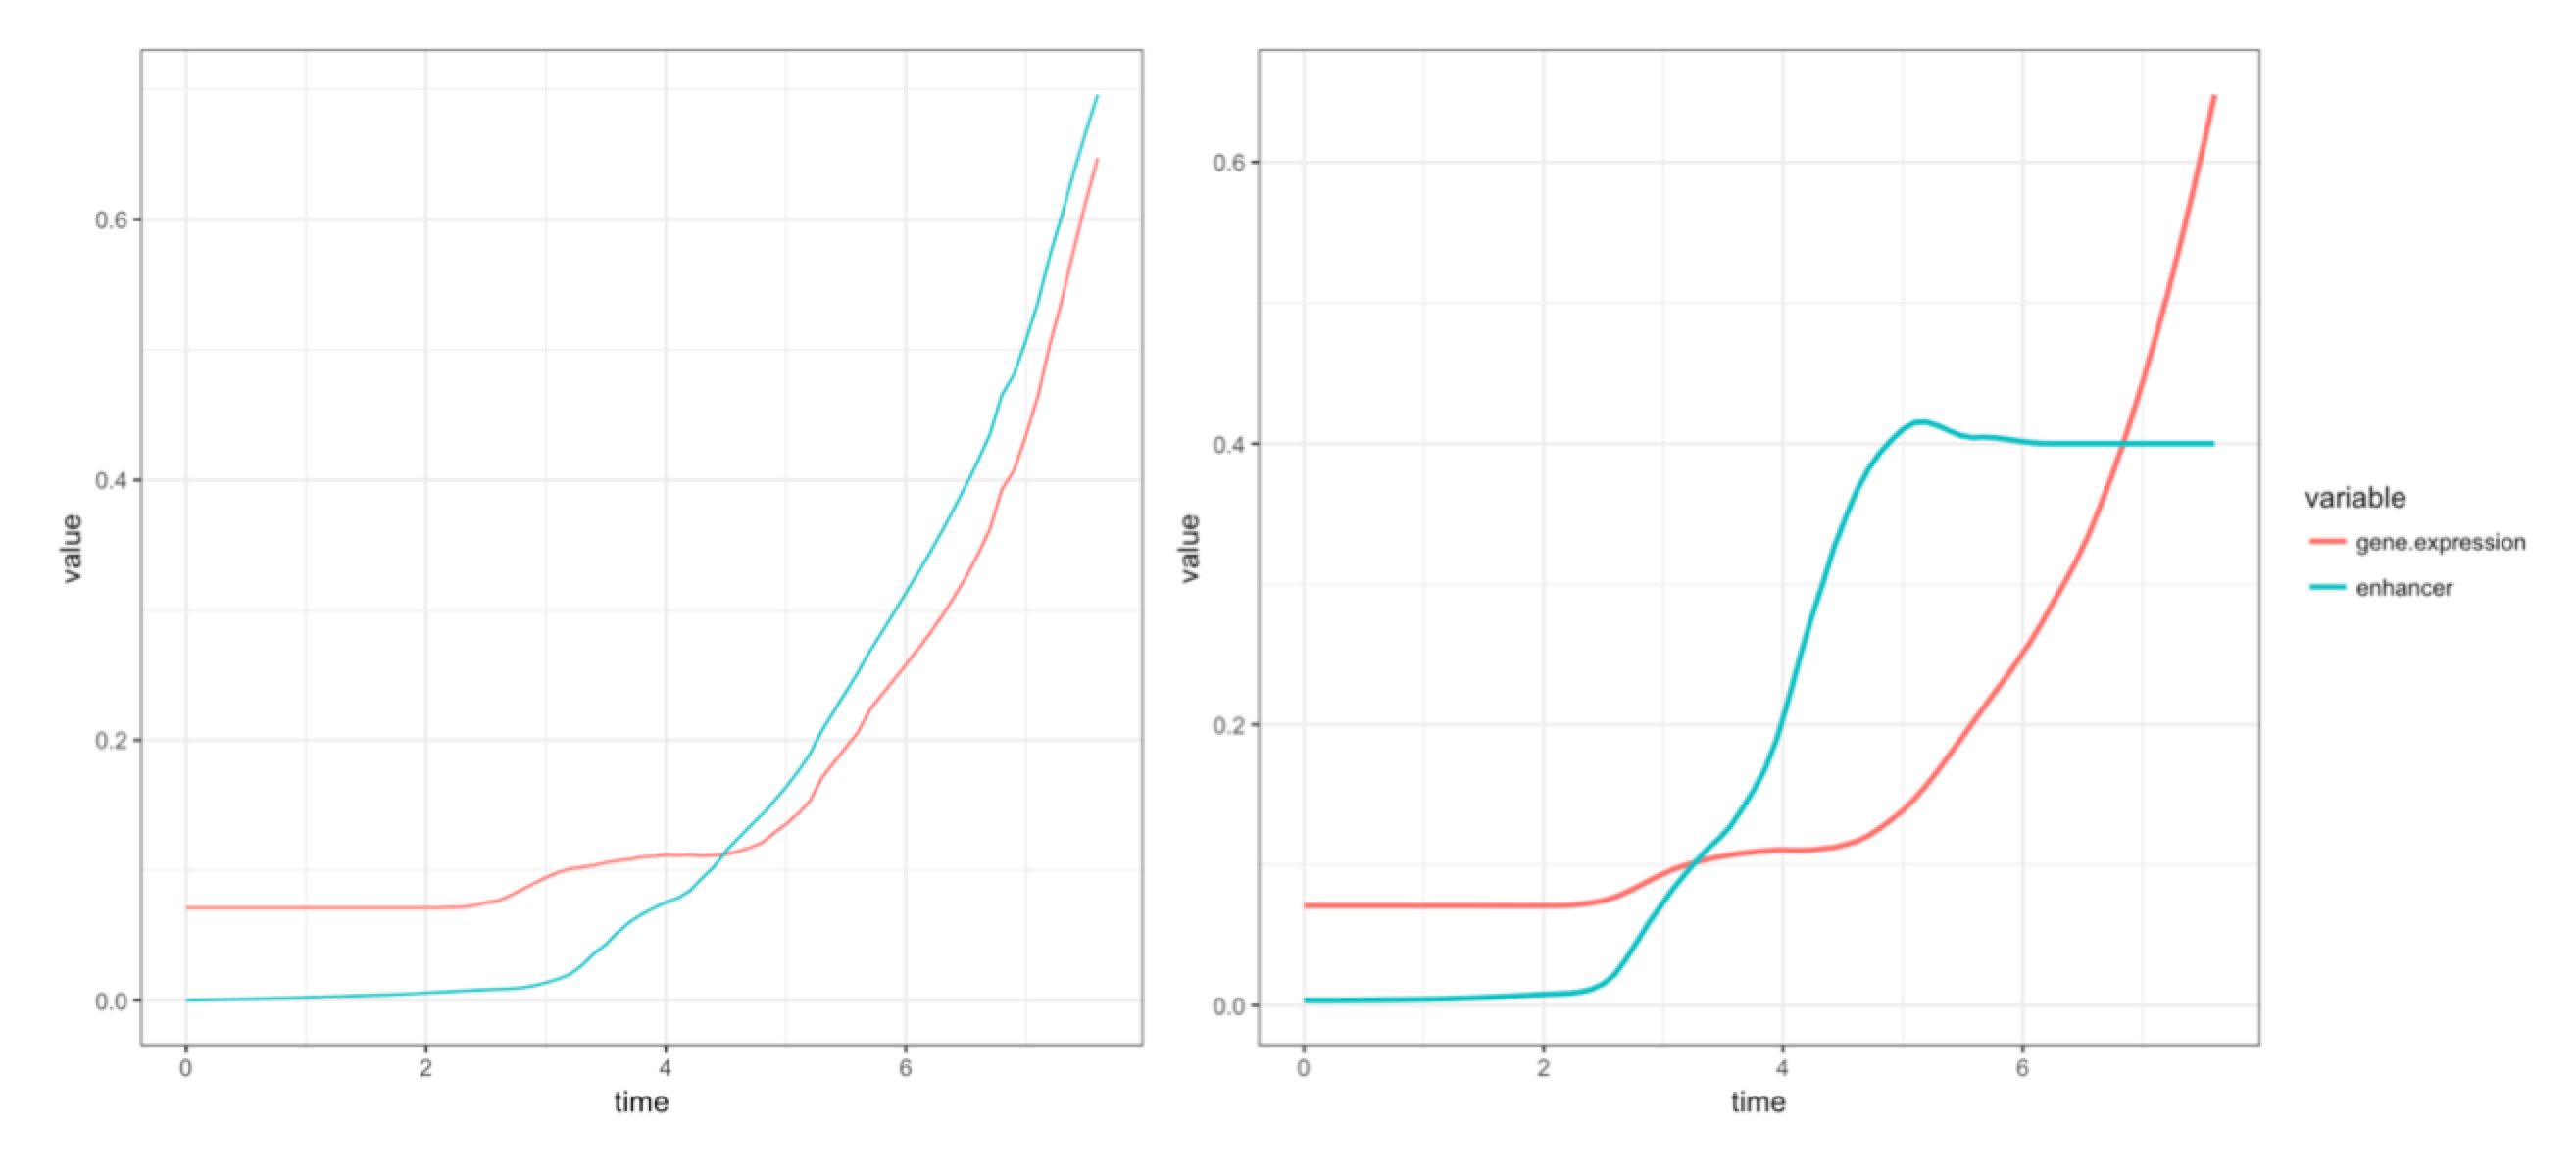
\includegraphics[width=\textwidth]{one.png}
    \caption{\textbf{To examples with varying enhancer-gene expression scores.} In the plot to the left, a gene-enhancer relationship shows a fast-activation. In the plot to the right, the enhancer becomes active but the regulatory process underlying the gene is relatively slow (i.e. a lag is observed.}
    \label{fig:one}
\end{figure}


\begin{figure}[ht]
    \centering
    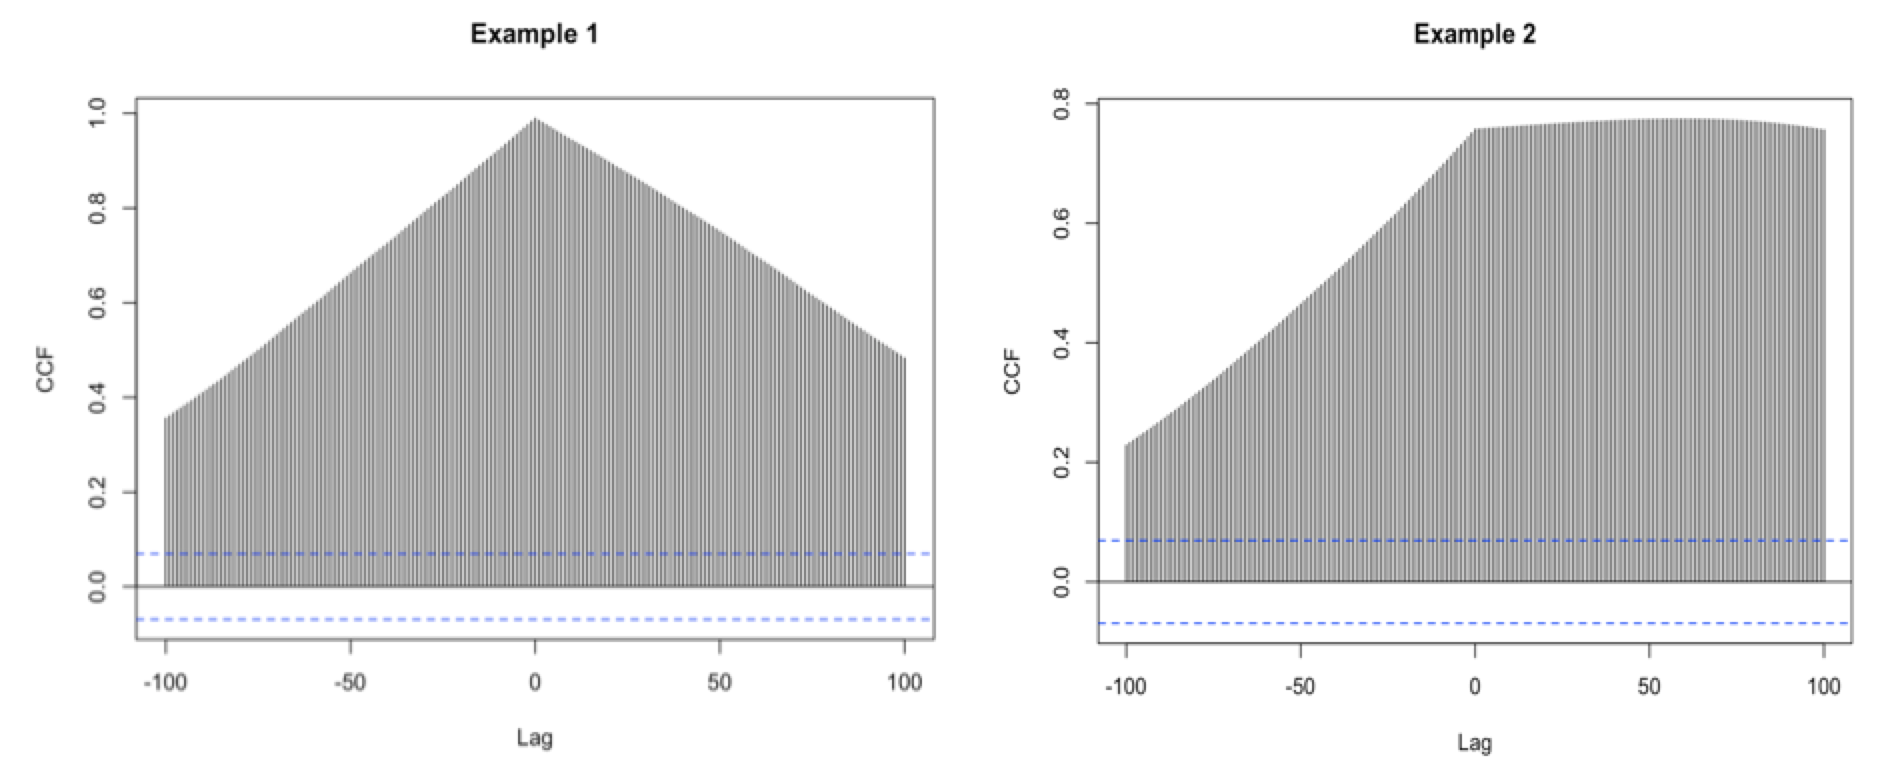
\includegraphics[width=\textwidth]{two.png}
    \caption{\textbf{Output plots from the \texttt{ccf} function}. The plot on the left verifies that the tighest correlation between the variables in Figure 2 (left) occurs with no lag in the variables. However, the maximized correlation for the example on the right occurs with a lag of $> 50$ units.} 
    \label{fig:two}
\end{figure}

\section*{Links to the BST245 Course}
\begin{itemize}
  \item Longitudinal data analysis
  \item Correlated correlated variables
\end{itemize}

\section*{R Packages/functions discussed}
\begin{itemize}
  \item \texttt{ccf}
  \item \texttt{forecast} (https://github.com/robjhyndman/forecast)
\end{itemize}



\end{document}
